\section{Experiments}

We devise a series of experiments to validate the methodology. In this section, we describe the experimental setup (Section~\ref{experiment_setup}), report results of the model evaluated through online (Section~\ref{online_demonstration}) and offline methods (Section~\ref{offline_eval}), and also perform ablation studies (Section~\ref{cap_ablation}). We use two tasks: alcohol bottle capping and brush flipping, and evaluate the full residual-imitation model against a classical optimization-based retargeting \cite{anyteleop} and pure imitation model-based retargeting.   

\subsection{Experimental Setup}
\label{experiment_setup}

\begin{figure}[ht]
    \centering
    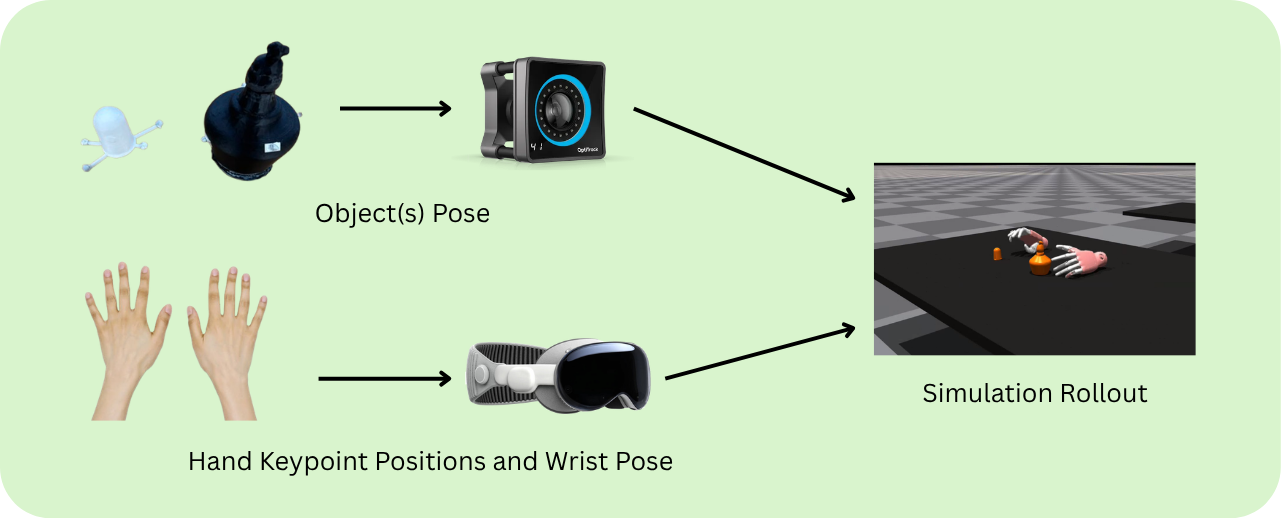
\includegraphics[scale=0.35]{../figures/data_collection_pipeline_horizontal.png}
    \caption{Overview of the data collection pipeline, showing how hand and object data flows from the Apple Vision Pro and OptiTrack systems through to the IsaacGym simulator.}
    \label{fig:data_collection_pipeline}
\end{figure}

As seen in \Cref{fig:data_collection_pipeline}, to collect training data or perform teleoperation, we use two systems, the Apple Vision Pro (AVP) and the OptiTrack. The simulator and data streaming runs at 60 Hz. Using the AVP SDK and VisionProTeleop \cite{visionproteleop}, we collect the 21 keypoints and wrist pose per hand, and with the OptiTrack, we record the object poses. The objects used are an alcohol burner and cap. They were sourced from the Oakink2 \cite{oakinkv2} dataset's mesh files, and modified to include the OpitTrack markers. The markers were placed on the objects in a manner that minimally affects the user's manipulation experience.

Since the two systems have different coordinate frames, we perform a calibration to map the two into a single frame by using a tracker on the tip of the index finger of the right hand. By moving the hand around in the workspace of the AVP and the OptiTrack we have a set of two points that we use the Umeyama \cite{umeyama} algorithm to map from the AVP to OptiTrack. The mapping is not perfect, which may be attributable to the image-based machine-learning techniques the Apple Vision Pro uses for finger and wrist pose estimation, and potentially different fingertip positions. We determined that the speed of the movements within the space had a positive linear correlation with the remapping error. Moving at a reasonable manipulation speed of around 200-300 $mm/s$, the RMSE between the systems was around 8-12 mm.


\paragraph{Teleoperation Architecture Pipeline}
\Cref{fig:live-pipeline} shows the live capture and teleoperation loop. The AVP and OptiTrack stream data at 60Hz, over WiFi and Ethernet respectively. The laptop fuses the two into a single frame --- the Umeyama AVP$\rightarrow$OptiTrack calibration places hands and objects in a common Motive frame, stamps it with a sequence number and capture time, and publishes it as
\texttt{msgpack} over a ZeroMQ \textsc{pub} socket at $60$\,Hz. The desktop subscribes and runs ManipTrans in Isaac Gym at roughly $60$\,Hz. Because the consumer runs below the publisher rate, the transport delivers the newest frame and discards the backlog rather than queueing it; a FIFO would let latency accumulate without bound across a teleoperation session. The desktop's rendered viewer
returns to the laptop over VNC at $15$\,Hz, closing the loop for the operator.

\begin{figure}[H]
  \centering
  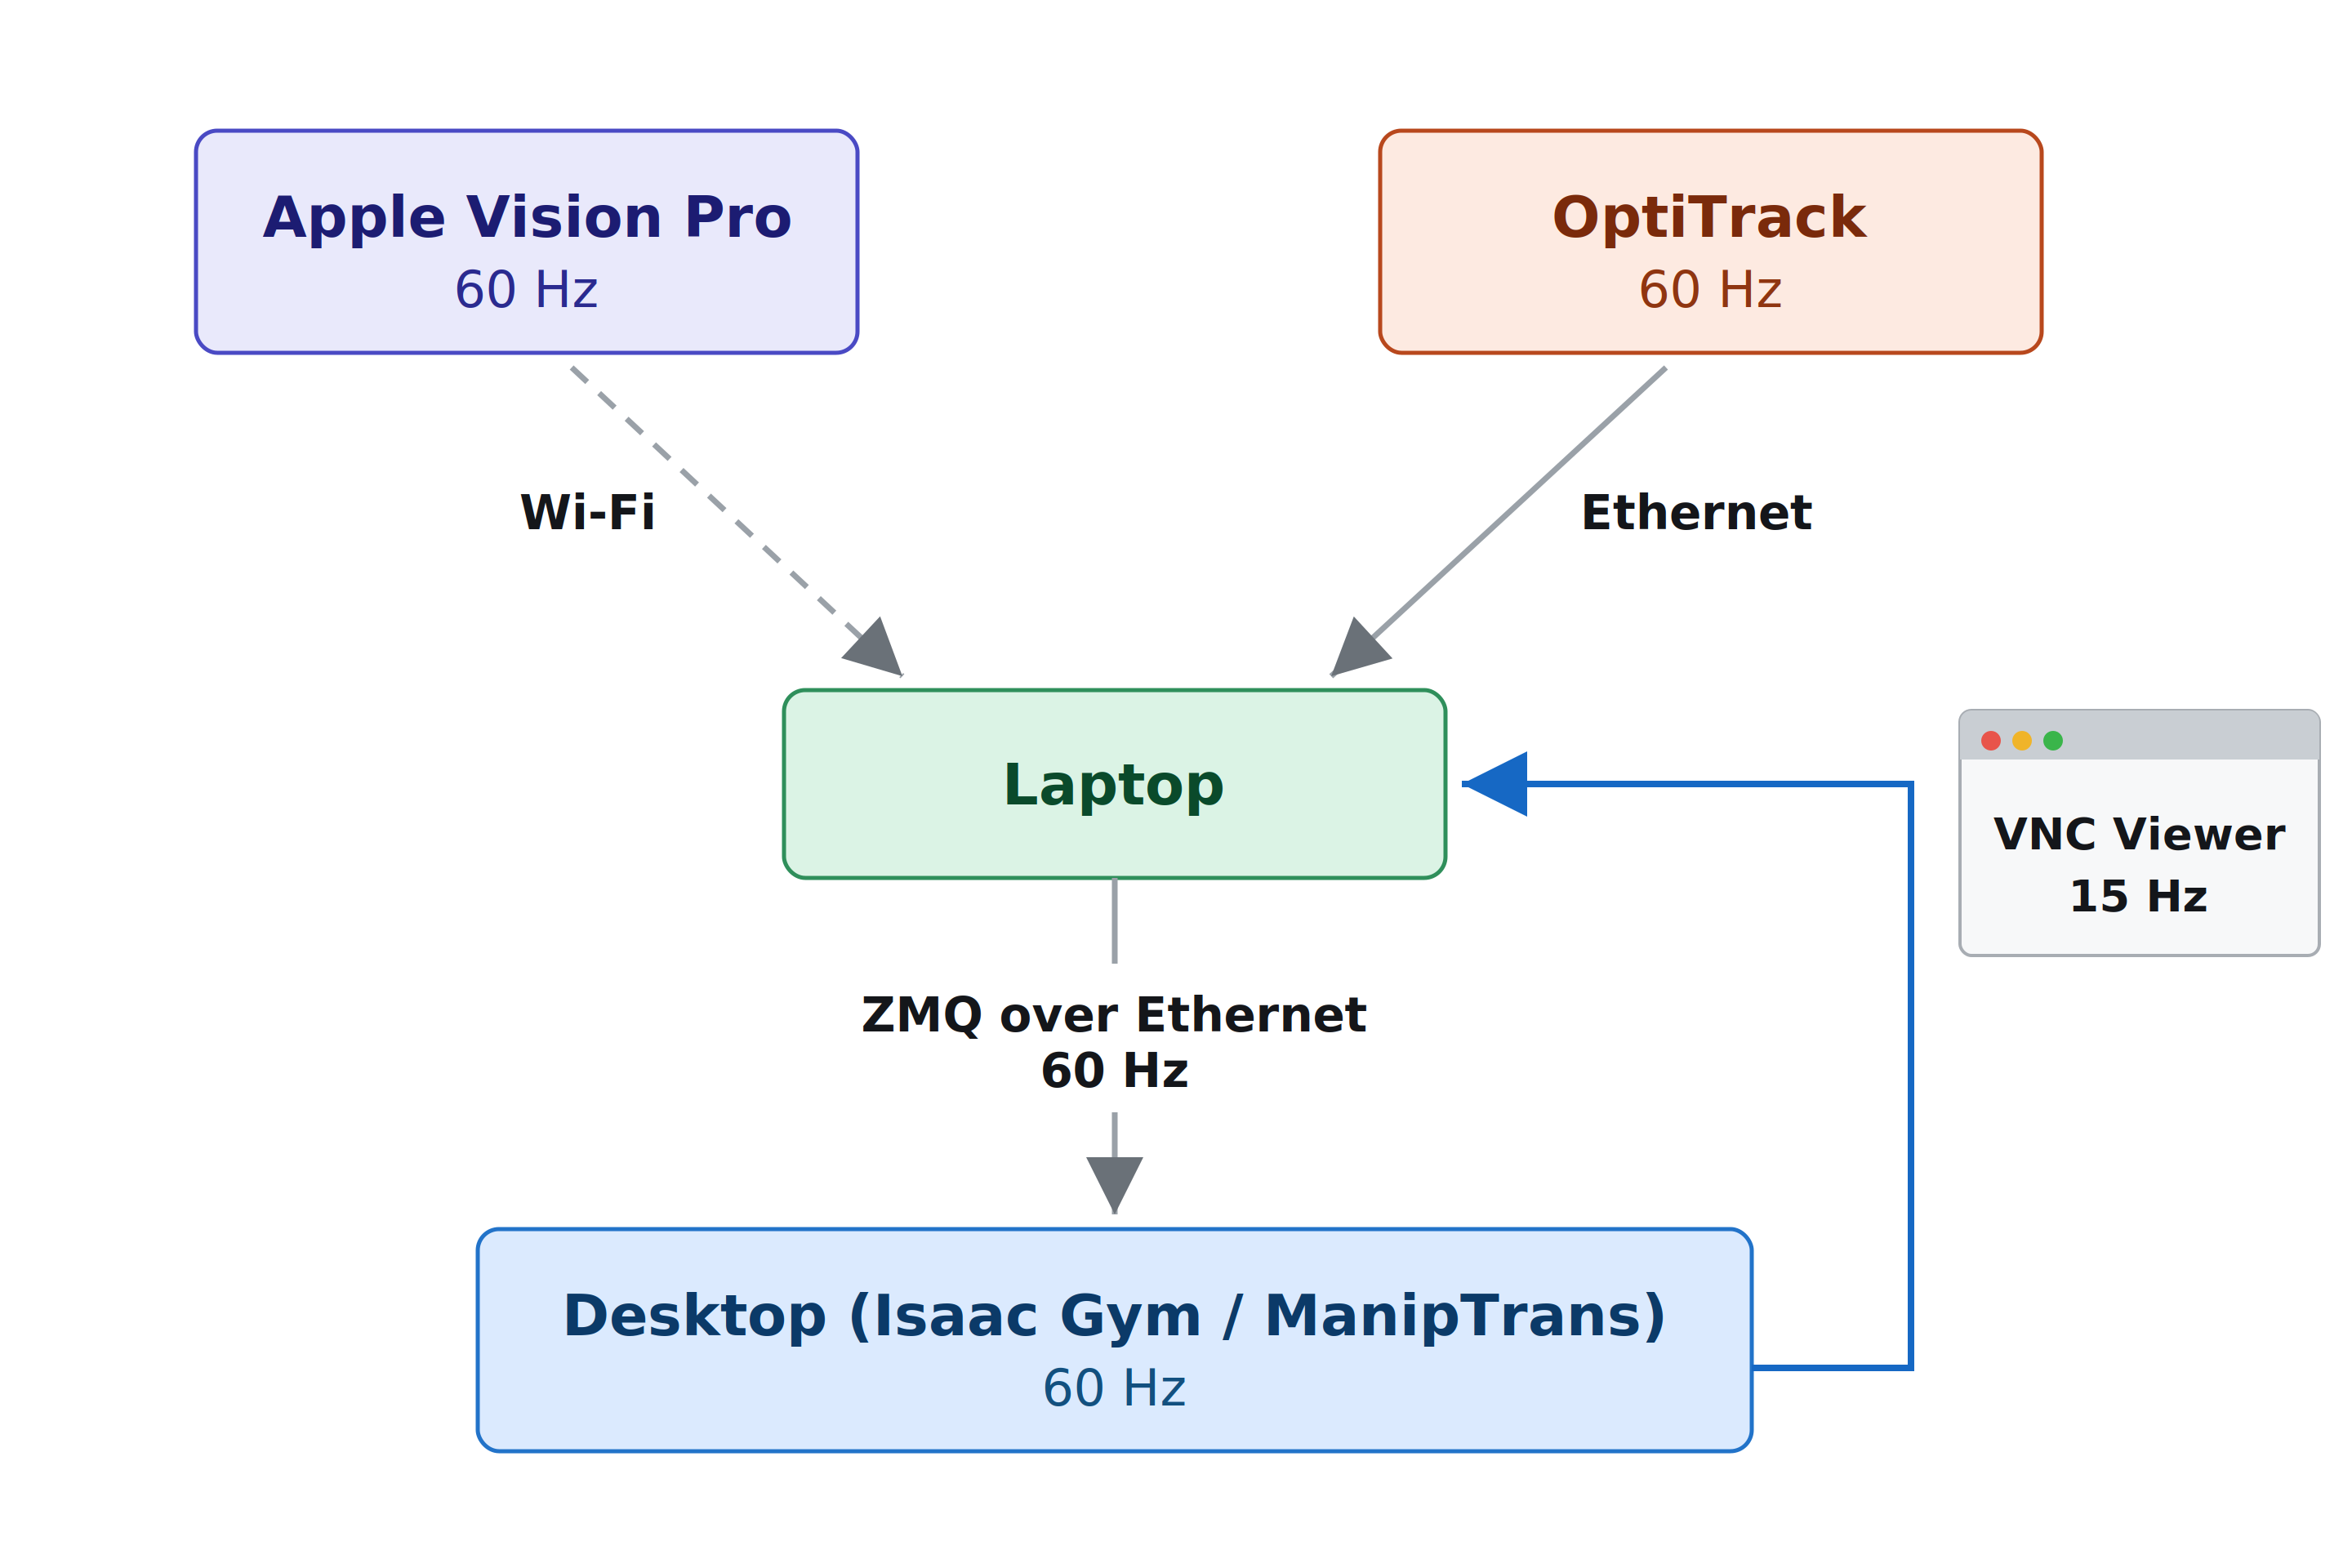
\includegraphics[scale=0.1]{figures/data_collection_pipeline_zmq_v11.png}
  \caption{Live capture and teleoperation pipeline. Rates are
  measured end-to-end latency.}
  \label{fig:live-pipeline}
\end{figure}

We train the residual module $R$ with the actor-critic PPO algorithm \cite{ppo}, optimized with Adam \cite{adam}; the full set of network and PPO hyperparameters is given in Tab.~\ref{tab:policy-hparams}. All simulation is carried out in Isaac Gym \cite{isaacgym}. Training is performed on an HPC cluster equipped with NVIDIA V100 and A100 GPUs, while evaluation, visualization, and teleoperation are run on a single NVIDIA RTX 4090 GPU.

\subsection{Data collection}

\paragraph{Demonstrations}

Both tasks embody real-world manipulation scenarios: the first involves capping an alcohol burner bottle of the kind found in a laboratory, and the second involves reorienting a brush. Both are illustrated in \Cref{fig:bottle_bc_task_breakdown}.

\begin{figure}[H]
    \centering
    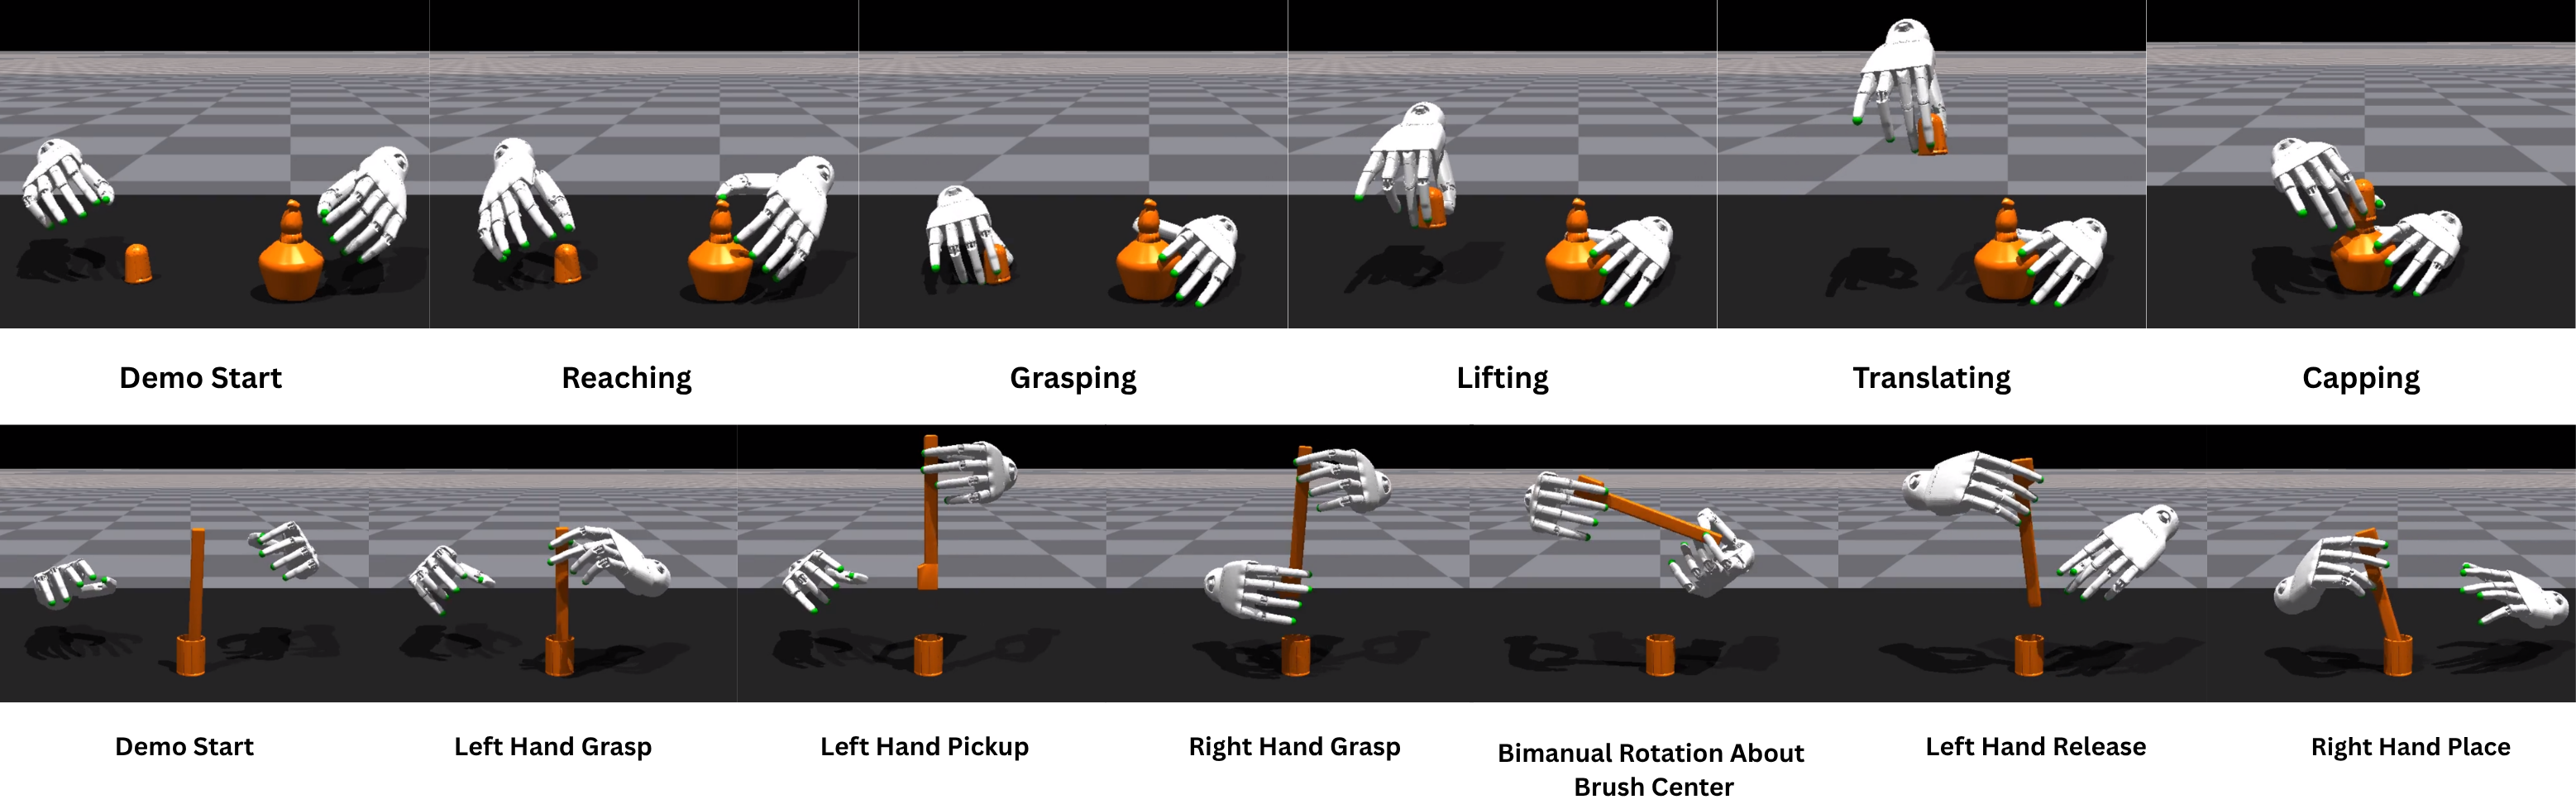
\includegraphics[scale=0.18]{../figures/bottle_bc_task_breakdown.png}
    \caption{The task decomposition of the bottle and brush cap manipulation task.}
    \label{fig:bottle_bc_task_breakdown}
\end{figure}

% \begin{figure}[ht]
%     \centering
%     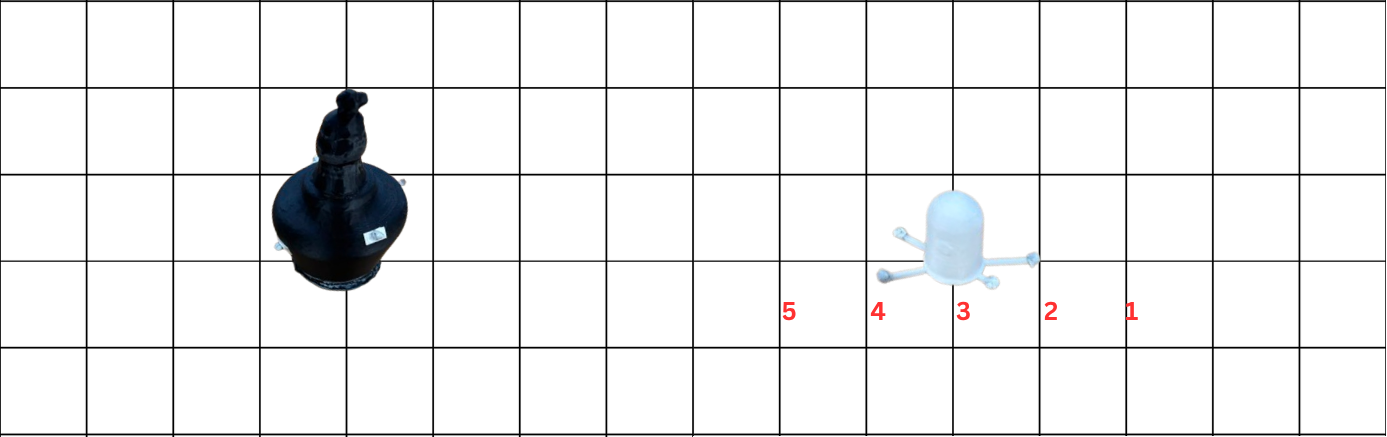
\includegraphics[scale=0.3]{../figures/bottle_cap_grid.png}
%     \caption{Grid to describe the setup for data collection. Five distinct starting positions are used.}
%     \label{fig:data_collection_grid}
% \end{figure}

\begin{figure}[H]
    \centering
    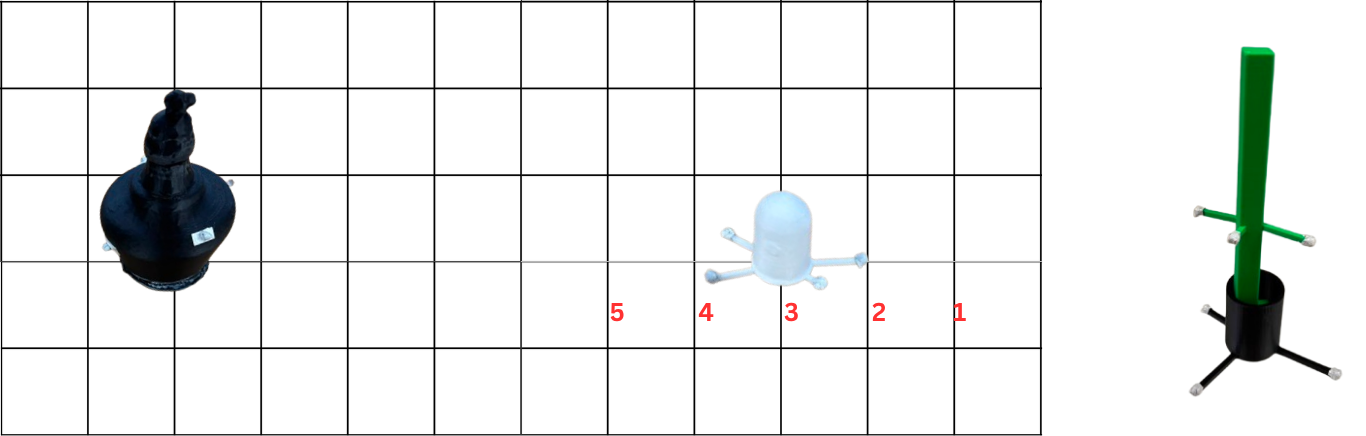
\includegraphics[scale=0.25]{../figures/bottle_bc_data_collection.png}
    \caption{The props used for data collection for the bottle capping and brush cup demonstration.}
    \label{fig:bottle_cap_brush_cup}
\end{figure}

To quantify the trajectories collected, we use a grid-based system to aid us in generating trajectories with as much similarity or difference as we would like. We collect trajectories from 5 distances away from the bottle body where the left hand holds the bottle body and the right hand grasps the cap. As seen in Fig. \ref{fig:bottle_bc_task_breakdown} Both hands start above the objects in a neutral position and reach towards them. The right hand picks up the cap and moves it towards the body, while the left hand stabilizes the bottle, and the demo terminates when the cap is seated on top of the bottle.

For the brush demonstration, we collect data such that the initial orientation of the brush is constant, and the trajectory is changed by lifting the brush to different heights and using different rotation speeds.
To encourage generalization we rotated the brush at different velocities. Similar to the bottle capping task, the hands start in a neutral palm facedown pose, the left hand grasps the end of the brush, lifts it up, then the right hand grasps the bristled end of the brush and both hands rotate the brush about the center point. Then the left hand releases the brush, and the right hand places it back into the cup.

\textbf{Data Augmentation}
For the bottle demonstration, we generate trajectories to increase the model generalizability. We apply affine transformations to the hand and/or objects across the entire trajectory. The transformations include rotations of the hand and bottle trajectories, which are applied using a matrix operation as seen in:
\begin{equation}
    \hat{A}_{\text{pose}}[\tau_k] = T_{\text{trans}} \cdot A_{\text{pose}}[\tau_k]
    \label{eq:pose_transform}
\end{equation}

\noindent Here, $A_{\text{pose}}[\tau_k]$ refers to the pose of either the hand or the object 
at the $k$-th frame of trajectory $\tau$. A rigid transformation $T_{\text{trans}} \in SE(3)$ 
is applied to each such pose, yielding the augmented pose $\hat{A}_{\text{pose}}[\tau_k]$.  



\subsection{Model Performance}

We perform a series of tests to motivate the need for training a more comprehensive model that can generalize to different tasks and a more informed algorithm than pure kinematic retargeting. Tests were performed both offline, by playing back demonstrations, and online, using a live teleoperation setup. To evaluate the online performance we use qualitative metrics, but online, we used quantitative and qualitative metrics. For qualitative evaluation, we ensured that the hand was manipulating the object with the same fingers used as the operator or demo. In some cases, the model learned to pinch the cap between the index and middle finger rather than between the thumb and index finger. For quantitative evaluation, we rollout the demonstration 128 times on a policy and capture the success rate, which is described below. 

\subsubsection{Evaluation Metrics}
\label{sec:metrics}

For offline demonstrations, we evaluate all conditions using three quantitative metrics following ManipTrans~\cite{maniptrans}, averaged over all successful rollouts with bimanual metrics computed per hand and averaged across both hands: \textbf{object translation error} $E_t = \frac{1}{T}\sum_{t=1}^{T}\|p^{\mathrm{tsl},t}_{\hat{o}} - p^{\mathrm{tsl},t}_{o}\|_2$ (cm), \textbf{object rotation error} $E_r = \frac{1}{T}\sum_{t=1}^{T}\|\log(R^{\mathrm{rot},t}_{\hat{o}}(R^{\mathrm{rot},t}_{o})^{-1})\|_2$ (degrees),  and \textbf{mean per-fingertip error} $E_{ft} = \frac{1}{T \cdot M}\sum_{t=1}^{T}\sum_{f=1}^{M}\|t^t_{d_f} - t^t_{h_f}\|_2$ (cm) over $M{=}2$ fingertip joints (index and thumb) because they are most used for the manipulation tasks. A rollout is successful if all three errors remain below the thresholds $E_r < 30^\circ$, $E_t < 3$\,cm, and $E_{ft} < 6$\,cm; for bimanual tasks both hands must satisfy all conditions simultaneously. The success rate (SR) is the fraction of successful rollouts per demonstration.

For online demonstrations, task success is evaluated qualitatively by visual inspection, with each task decomposed into subtasks and completion assessed at the phase level.

%%%%%%%%%%%%%%%%%%%%%%%%%%%%%%%%%%%%%%%%%%%%%%%%%%%%%%%%%%%%%%%%%%%%%%%%%%%%%%%%%%%%%%%%%%%%%%%%%%%%%%%%%%%%%%%%
% ____________________________________________ EXPERIMENTAL RESULTS __________________________________________ %
% ____________________________________________________________________________________________________________ %
% ____________________________________________________________________________________________________________ %
% ____________________________________________________________________________________________________________ %
% ____________________________________________________________________________________________________________ % 
% ____________________________________________________________________________________________________________ %

\section{Experimental Results}
\subsection{Offline Demonstration}
\label{offline_eval}

\paragraph{Cross-validation protocol.}
The $50$ reach demonstrations, $10$ at each of five reach distances, are partitioned into five
folds by a deterministic stratified split: demonstrations are grouped by distance and
dealt two per distance to each fold, so every fold holds out $10$ demonstrations spanning all five
distances and trains on the remaining $40$. For each fold we score $128$ completed episodes. An
episode counts as a success if it reaches the final demonstration frame with both hands never
exceeding the evaluation tolerances --- $6$~cm thumb- and index-tip tracking error, $3$~cm object
position error and $45^\circ$ object orientation error. The success rate of a demonstration is the fraction of its scored episodes that succeed; each cell of Tab.~\ref{fig:kfold_confusion_matrix} averages the two demonstrations that fall in that (fold, distance) pair, with marginal means over folds and over distances.

\begin{figure}[H]
    \centering
    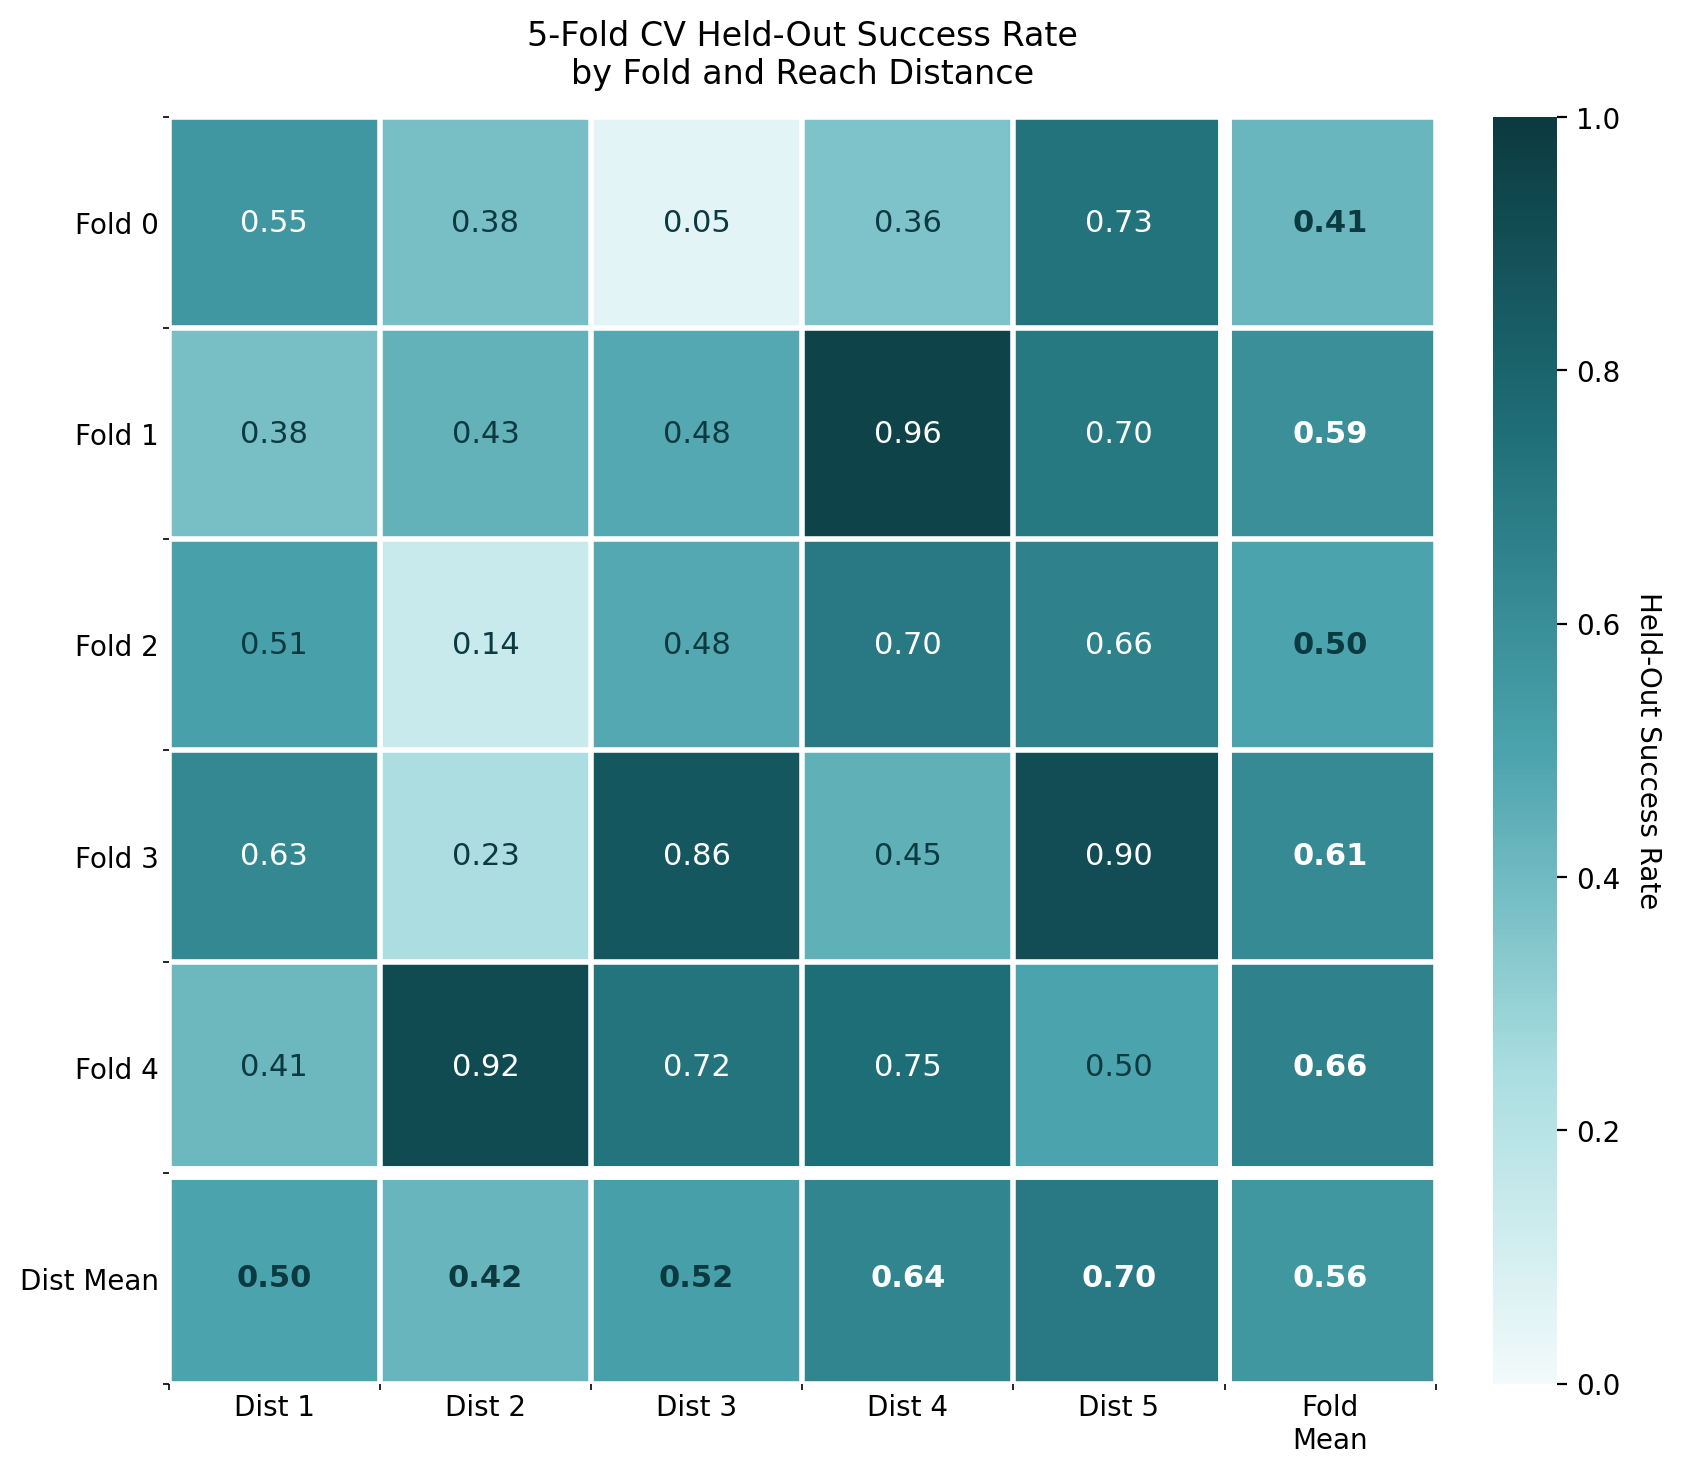
\includegraphics[scale=0.4]{../figures/kfold_confusion_matrix_v2.png}
    \caption{K-fold matrix results describing the success rate per fold and per demonstration distance.}
    \label{fig:kfold_confusion_matrix}
\end{figure}

We notice that some of the demonstrations have very low success rates, and in many of the cases, this is due to a failure of the initial grasp, or a grasp that is unstable so the cap falls out from the fingertips out side. Notably, there seems to be a trend of improvement as the distance decreases. This could be attributed to the hands are closer to the AVP, which could lead to a more accurate retargeting. 

\subsubsection{Bottle Capping task}

We compare the results of the offline rollout to the kinematic retargeting imitation only policy and a pure optimization based method Dex-retargeting \cite{anyteleop}. To understand overall performance at a granular level, we decompose the task by hand and phase. We evaluate the phase-level success counts over 10 zero-shot
demonstrations for both the bottle capping and the brush-cup demonstrations.

The results in Table~\ref{tab:task_breakdown} reveal that the imitator's failures
are concentrated entirely in the right hand's active manipulation phases.
While both models reach the bottle and cap successfully (10/10) and the left hand
stabilizes the bottle in all cases, the imitator grasps the cap in only 2 out of
10 demonstrations and fails to lift or seat it in any.
This is expected: the imitator tracks the kinematic reference trajectory but has no
mechanism to respond to contact forces or object resistance.
When the right hand closes around the cap, the fingers reach the reference joint
angles but without contact-aware correction, the fingertips fail to generate
sufficient grip force to lift the cap.
The two successful grasps are likely attributable to favorable initialization
geometry rather than a robust contact strategy.

The residual policy recovers this gap by conditioning on fingertip contact forces
and hand-to-object distances, allowing it to actively adjust joint targets as the
fingers approach and close around the cap.
This is reflected in the results: 8/10 demonstrations successfully grasp, lift,
and translate the cap.
The single additional failure at seating (7/10 vs.\ 8/10) is consistent with
the task's most contact-critical moment --- placing the cap requires simultaneously
maintaining grip and applying downward force, so a single lost contact at this
stage results in failure.

\begin{table}[h]
    \centering
    \begin{tabular}{llccc}
        \toprule
        \textbf{Hand} & \textbf{Phase} & \textbf{Imitator} & \textbf{Residual (ours)} & \shortstack{\textbf{Optimization-Based}\\\textbf{Retargeting}} \\
        \midrule
        \multirow{2}{*}{Left}
            & Reach bottle       & 10 / 10 & 10 / 10 & 10 / 10 \\
            & Stabilize bottle   & 10 / 10 & 10 / 10 & 10 / 10 \\
        \midrule
        \multirow{5}{*}{Right}
            & Reach cap          & 10 / 10 & 10 / 10 & 10 / 10 \\
            & Grasp cap          &  0 / 10 & 10 / 10 & 10 / 10 \\
            & Lift cap           &  0 / 10 &  8 / 10 & 10 / 10 \\
            & Translate cap      &  0 / 10 &  8 / 10 & 10 / 10 \\
            & Seat cap           &  0 / 10 &  7 / 10 &  0 / 10 \\
        \bottomrule
    \end{tabular}
    \caption{Phase-level success counts over 10 zero-shot demonstrations,
             broken down by hand and task phase.}
    \label{tab:task_breakdown}
\end{table}

\paragraph{Cap-Scaling Ablations}
\label{cap_ablation}

\begin{figure}
    \centering
    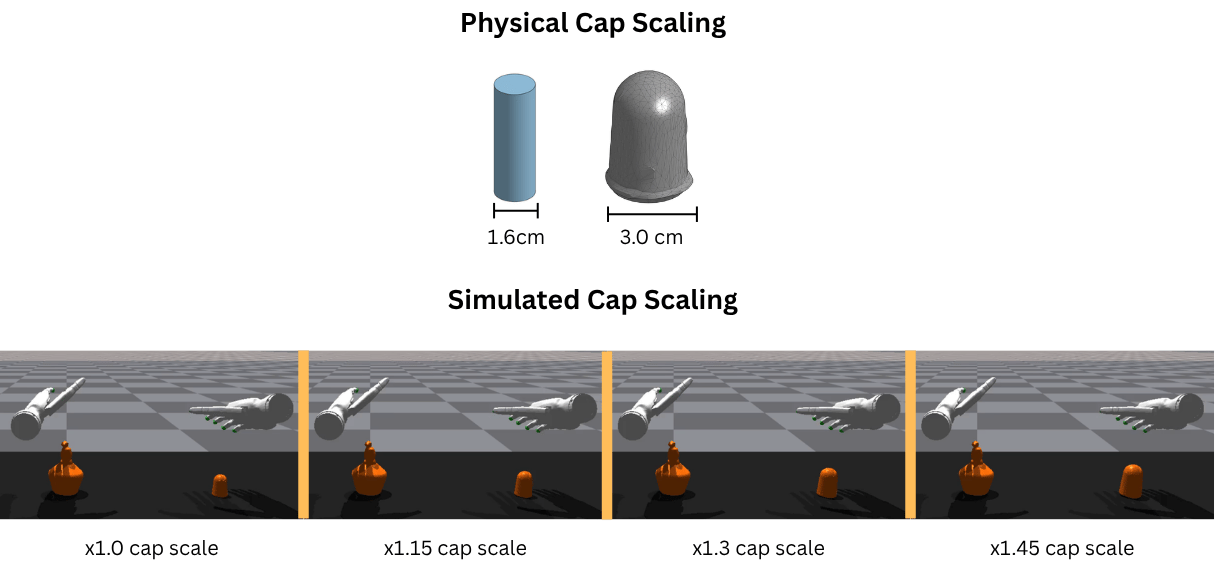
\includegraphics[scale=0.23]{../figures/physical_simulated_cap_scaling.png}
    \caption{Physical cap ablation: outer diameter reduced by 1.4\,cm, and simulated cap ablation by scaling the mesh size.}
    \label{fig:physical_simulated_cap_ablation}
\end{figure}

To motivate the need to assist the imitation model with contact force, we performed
an ablation study that injects contact force by scaling the cap using both physical
and software methods. To improve the pinching capability of the imitator, we designed
a thinner cap with an outer diameter of 1.6\,cm, compared to roughly 3.0\,cm for the
original. Evaluating the manipulation task with the imitator over 10 demonstrations,
we observe improved performance. While the improvement is substantial, failures
persist, arising from the policy's limited understanding of the task rather than from
grasp geometry alone.

We combine this with software-based ablations by scaling the cap mesh by up to
1.45$\times$; results for the right hand are reported in
\Cref{tab:cap_ablation}.

\begin{table}[H]
    \centering
    \begin{tabular}{llcccc}
        \toprule
        \textbf{Model} & \textbf{Phase} & $\times$\textbf{1.00} & $\times$\textbf{1.15} & $\times$\textbf{1.30} & $\times$\textbf{1.45} \\
        \midrule
        \multirow{5}{*}{\shortstack[l]{Optimization-Based\\Retargeting}}
            & Reach cap     & 13 / 13 & 13 / 13 & 13 / 13 & 13 / 13 \\
            & Grasp cap     & 11 / 13 & 12 / 13 & 13 / 13 & 12 / 13 \\
            & Lift cap      & 10 / 13 & 12 / 13 & 13 / 13 & 11 / 13 \\
            & Translate cap &  9 / 13 & 11 / 13 & 12 / 13 & 10 / 13 \\
            & Seat cap      &  0 / 13 &  1 / 13 &  1 / 13 &  1 / 13 \\
        \midrule
        \multirow{5}{*}{Pre-Trained Imitator}
            & Reach cap     & 13 / 13 & 13 / 13 & 13 / 13 & 13 / 13 \\
            & Grasp cap     &  3 / 13 &  8 / 13 &  9 / 13 &  8 / 13 \\
            & Lift cap      &  3 / 13 &  5 / 13 &  6 / 13 &  5 / 13 \\
            & Translate cap &  3 / 13 &  4 / 13 &  5 / 13 &  4 / 13 \\
            & Seat cap      &  1 / 13 &  3 / 13 &  4 / 13 &  3 / 13 \\
        \midrule
        \multirow{5}{*}{Fine-Tuned Residual (ours)}
            & Reach cap     & 13 / 13 & 13 / 13 & 13 / 13 & 13 / 13 \\
            & Grasp cap     & 13 / 13 & 13 / 13 & 13 / 13 & 12 / 13 \\
            & Lift cap      & 12 / 13 & 13 / 13 & 13 / 13 & 12 / 13 \\
            & Translate cap & 11 / 13 & 12 / 13 & 12 / 13 & 11 / 13 \\
            & Seat cap      & 10 / 13 & 11 / 13 & 12 / 13 & 10 / 13 \\
        \bottomrule
    \end{tabular}
    \caption{Phase-level success counts over 13 demonstrations for each model across four cap diameter scales. $\times 1.00$ corresponds to the original cap mesh size reported in Table~\ref{tab:task_breakdown}.}
    \label{tab:cap_ablation}
\end{table}

What is observed is that the thinner cap along itself improves the performance of the pre-trained imitator model, as there is one demonstration that can seat the cap. However, we can see a large improvement with the thinner cap and the scaled model inside the simulation. The largest jump is between x1.0 and x1.15 where the seating of the cap for the imitator model goes from 1 to 4. Overall we can see that the scaling of the cap best improves the performance of the imitator model, which makes sense, as it is the least accurate at performing the kinematic retargeting. There also seems to be a general improvement in performance up until x1.3, and at x1.45 times, the performance decreases. Another observation is the performance of the fine-tuned residual model performs worse when the cap gets too large. At x1.45 scale, the performance decreases across the grasping, lifting, translation, and seating. This could be attributed to a too-large distribution shift of the demonstration compared to the training data.  

\subsubsection{Cup Brush} 

The results in \Cref{tab:brush_task_breakdown} reveal a sharp contrast between the two learned policies. The imitator completes the initial left-hand reach in all ten demonstrations but fails at every subsequent phase, never once achieving a stable grasp. The failure mode is consistent across all trials: the fingertips approach the brush but do not close around it. We attribute this to two factors. First, the retargeted fingertip positions carry a residual error relative to the ground-truth human fingertip trajectories, and because grasping is highly sensitive to millimeter-scale fingertip placement, even a small offset is sufficient to leave the digits short of the object surface. Second, the imitator is trained purely on kinematic targets and receives no contact or force feedback, so it has no signal with which to detect that a grasp has not been established and no mechanism to correct the closure online. The policy therefore executes an open-loop approximation of the demonstrated motion and proceeds as if the object were held.

The residual policy completes the full sequence in five of ten demonstrations, with the remaining failures distributed across the later phases rather than concentrated at the grasp. Critically, the failures are no longer concentrated at the grasp: the corrective term is sufficient to close the fingers around the brush in nine of ten trials, and the remaining errors are distributed across the later, more constrained phases. Two distinct failure mechanisms account for the losses. The first is grasp quality. One demonstration fails outright at the left-hand lift, and a second establishes a poor grasp that only manifests later, during the right-hand reach, when the brush is no longer held securely enough for the second hand to engage it. The second and dominant mechanism is the handover itself. In two demonstrations the left hand fails to release cleanly after the bi-manual rotation and remains caught on the brush, blocking the transfer. Notably, these two demonstrations have a grasp that is lower on the brush, which causes the left hand release to fail. A
further demonstration completes the release but strikes the rim of the cup during seating, so the brush is never inserted. The bi-manual rotation phase itself incurs no additional failures, indicating that once a secure two-handed configuration is reached, the reorientation is reliable. The bottleneck lies instead at the transitions into and out of that configuration, where fine control of contact release and terminal placement is required — precisely the regime in which the
residual correction, trained without explicit contact feedback, has the least to work with.

The optimization-based retargeter shares the imitator's fundamental limitation at the grasp: the vector-based objective optimizes for a different quantity than fingertip alignment, so the left hand frequently collides with or fails to contact the brush rather than closing around it. Unlike the imitator, this failure is recoverable in a live teleoperation setting where the operator can compensate online, but in the offline rollout evaluated here there is no such corrective mechanism, and the method does not progress beyond the initial reach.

\begin{table}[H]
    \centering
    \begin{tabular}{llccc}
        \toprule
        \textbf{Phase} & \textbf{Hand} & \textbf{Imitator} & \textbf{Residual (ours)} & \shortstack{\textbf{Optimization-Based}\\\textbf{Retargeting}} \\
        \midrule
        Reach    & Left     & 10 / 10 & 10 / 10 & 10 / 10 \\
        Lift     & Left     &  0 / 10 &  9 / 10 & 0 / 10 \\
        Reach    & Right    &  0 / 10 &  8 / 10 & 0 / 10 \\
        Rotation & Bimanual &  0 / 10 &  8 / 10 & 0 / 10 \\
        Release  & Left     &  0 / 10 &  6 / 10 & 0 / 10 \\
        Seat     & Right    &  0 / 10 &  5 / 10 & 0 / 10 \\
        \bottomrule
    \end{tabular}
    \caption{Phase-level success counts over 10 zero-shot demonstrations of the
             brush-flipping task, broken down by task phase and hand.}
    \label{tab:brush_task_breakdown}
\end{table}

\subsection{Online Demonstration}
\label{online_demonstration}

We further develop the need of the generalized model through testing in teleoperation. We collect 10 consecutive trajectories from each distance, for a total of 50 demonstrations to generate the metrics below for both tasks. The success metric is fully determined qualitatively by evaluating the progress through the task.

\subsubsection{Bottle Capping Teleoperation}

\begin{table}[H]
    \centering
    \begin{tabular}{llccc}
        \toprule
        \textbf{Hand} & \textbf{Phase} & \shortstack{\textbf{Optimization-Based}\\\textbf{Retargeting}} & \textbf{Imitator} & \textbf{Residual (ours)} \\
        \midrule
        \multirow{2}{*}{Left}
            & Reach bottle       & 10 / 10 & 10 / 10 & 10 / 10 \\
            & Stabilize bottle   & 10 / 10 & 10 / 10 & 10 / 10 \\
        \midrule
        \multirow{5}{*}{Right}
            & Reach cap          & 10 / 10 & 10 / 10 & 10 / 10 \\
            & Grasp cap          &  7 / 10 & 10 / 10 &  9 / 10 \\
            & Lift cap           &  7 / 10 &  1 / 10 &  9 / 10 \\
            & Translate cap      &  6 / 10 &  0 / 10 &  8 / 10 \\
            & Seat cap           &  0 / 10 &  0 / 10 &  5 / 10 \\
        \bottomrule
    \end{tabular}
    \caption{Phase-level success counts over 10 consecutive teleoperation demonstrations at demonstration distance 5, broken down by hand and task phase.}
    \label{tab:online_teleop_success}
\end{table}

Qualitatively, the manipulation of the cap using the residual model requires the least amount of user feedback. The grasping and capping, the most interaction-heavy parts of the trajectory were assisted by the model. However, this model is unstable, and going out of distribution resulted in catastrophic spinning of the hands at high velocity. The dex-retargeting approach was the second most difficult to operate. While grasping was completed nearly every time, the cap would frequently rotate during the pinching grasp due to the sensitivity of the method to finger closing coordination. Because the operator hand pose is mapped directly to robot joint targets without contact-aware correction, the timing at which individual fingertips contact the cap surface is determined entirely by the operator's motion. If the index finger and thumb do not close at the same rate, one fingertip contacts the cap before the other, generating an asymmetric force that causes the cap to tilt or rotate rather than be gripped stably. This forces the operator to compensate by rotating the entire wrist, making seating the cap nearly impossible. Attempting to mitigate this with a three-finger grasp did not improve reliability; introducing a third finger increases the number of pairwise contact timing
differences from one to three, making synchronized contact even harder to achieve in practice. This suggests that pure kinematic retargeting is fundamentally limited for precision grasping tasks, as it places the full burden of contact coordination on the operator rather than the policy.

Finally, the ManipTrans imitation-only model demonstrates the weakest performance during teleoperation, with only a few successful instances of grasping the cap. The fundamental limitation is that the imitator reproduces the reference trajectory kinematically but produces only coarse positional targets, without the fine-grained fingertip precision required for contact-critical manipulation. The coarse positional targets produced by the imitator are sufficient for reaching the general vicinity of the cap, but not precise enough to bring the fingertips into contact with it, so the grasp is never established. This is consistent with the offline results in Table~\ref{tab:task_breakdown}, where the imitator achieves 0/10 grasps, and confirms that coarse kinematic imitation alone is insufficient for precision grasping tasks.


\begin{table}[H]
\centering
\begin{tabular}{lccccc}
\toprule
\textbf{Failure Mode} & \textbf{Dist. 1} & \textbf{Dist. 2} & \textbf{Dist. 3} & \textbf{Dist. 4} & \textbf{Dist. 5} \\
\midrule
Missed Grasp & 0 & 2 & 1 & 1 & 1 \\
Missed Translate & 0 & 0 & 2 & 0 & 1 \\
Missed Cap & 1 & 2 & 3 & 2 & 3 \\
Failed Lift & 1 & 0 & 0 & 0 & 0 \\
\midrule
\textbf{Total} & 2 & 4 & 6 & 3 & 5 \\
\bottomrule
\end{tabular}
\caption{Breakdown of residual-based teleoperation failure modes for the bottle-capping task across the five demonstration distances, aggregated over ten trials per distance.}
\label{tab:bottle_failure_modes}
\end{table}

Quantitatively, we observe that demonstration distance itself does not correlate with teleoperation failure rate; rather, performance is primarily determined by task phase. The initial grasp and final seating phases account for the largest share of failures, with the residual policy dropping from fifty out of fifty successes at the reach phase to thirty out of fifty by the seating phase. This indicates that the precision required to align fingers to the cap’s radius during grasping, and to align the cap’s descent point with the bottle opening during seating, are the two dominant bottlenecks in the teleoperation pipeline, rather than any degradation from operator distance or trajectory novelty.

\paragraph{Residual Model Performance}

Two qualitative failure modes were observed during live teleoperation, both consistent with distribution shift. First, when the operator deliberately slows or pauses their movements, for instance, while visually cross-referencing the simulated hand against the real one, the resulting
frame-to-frame deltas fall outside the velocity distribution the policy was trained on, pushing the observation out of distribution and increasing the likelihood of failure. Second, the policy becomes noticeably less stable during the capping phase at the end of the episode. We attribute
this to occlusion: as the two hands converge on the burner they increasingly obscure one another and the object, degrading the headset's keypoint estimates at precisely the moment the tracking targets must be most accurate. Training offers no exposure to this failure, since the keypoint noise in the augmentation pipeline is a single fixed offset per demonstration variant rather than a transient per-frame corruption. Together these suggest that the policy's robustness to variation in
demonstrated trajectories does not extend to variation in motion speed or to degraded target quality, and that operator guidance, per-step target noise, and training-time augmentation across a wider range of speeds would improve reliability in practice.


% \paragraph{Out of Distribution Motions}

% We evaluate the robustness of the bottle-capping policy by injecting out-of-distribution motions at teleoperation time: grasping and dropping the cap, vertical translation of the hand, lateral translation, grasping with the middle finger and thumb rather than the index and thumb, and throttling of the frame rate.

% We evaluate the effect of control frequency on policy performance by throttling the frame rate below the training frequency of \SI{60}{\hertz}. Performance degrades monotonically as the frame rate decreases. This is attributable to a distribution shift: the policy was trained on observations where fingertip positions, object poses, and wrist deltas are computed at \SI{60}{\hertz}, so the magnitude of per-frame $\Delta p$ and $\Delta \theta$ are implicitly encoded in the learned weights. At lower frequencies, the inter-frame displacements are larger, pushing the observation distribution outside the training support and causing the policy to produce incorrect corrections. This suggests that for real deployment, the teleoperation pipeline must maintain a consistent \SI{60}{\hertz} loop, and that frequency-robust training via frame rate randomization during training could be a promising direction for
% future work.

\subsubsection{Cup Brush Teleoperation}

\begin{table}[H]
    \centering
    \begin{tabular}{llccc}
        \toprule
        \textbf{Phase} & \textbf{Hand} & \textbf{Imitator} & \textbf{Residual (ours)} & \shortstack{\textbf{Optimization-Based}\\\textbf{Retargeting}} \\
        \midrule
        Reach    & Left      & 10 / 10 & 10 / 10 &  8 / 10 \\
        Lift     & Left      &  0 / 10 & 10 / 10 &  7 / 10 \\
        Reach    & Right     &  0 / 10 &  9 / 10 &  5 / 10 \\
        Rotation & Bi-manual &  0 / 10 &  4 / 10 &  0 / 10 \\
        Release  & Left      &  0 / 10 &  3 / 10 &  0 / 10 \\
        Seat     & Right     &  0 / 10 &  0 / 10 &  0 / 10 \\
        \bottomrule
    \end{tabular}
    \caption{Phase-level success counts over 10 teleop demonstrations of the
             brush-flipping task, broken down by task phase and hand.}
    \label{tab:teleop_brush_cup}
\end{table}

For the cup-brush task, the imitator model proves ineffective throughout, as the mapping between the demonstrated hand pose and the robot's joint targets is not precise enough to establish any manipulation capability. In every trial, the fingertips approach the brush but fail to close around it, so no phase beyond the initial reach is ever completed. The optimization-based retargeting approach performs better, reaching and lifting the brush in 8 and 7 out of 10 trials respectively, but fails to complete the rotation in any trial. The grasping and rotation are unintuitive to operate under this method, since the retargeter optimizes a separate objective from the manipulation goal directly, requiring constant operator correction that slows execution considerably. The residual model is the most capable of the three, successfully reaching and lifting in all trials and completing the rotation in 4 out of 10, but no method succeeds at seating the brush. A key difficulty is that the rotation phase requires the fingers to maintain contact with the brush while simultaneously allowing it to rotate between them — a regime in which simulated friction and contact dynamics may not accurately reflect real-world behaviour. The longer horizon of this task relative to bottle capping compounds these difficulties, as errors accumulate 
across phases and leave less margin for recovery at the terminal seating step.